\textbf{Verificación subsistema 1}

Como se mencionó en el apartado anterior, el menú desplegado en la interfaz presenta tres opciones y para comprobar que cada una funciona de manera correcta, se realizaron varias pruebas.

Para probar el monitoreo del proceso, se ejecutaron los distintos procesos de forma aislada, es decir se programó una rutina de calentamiento durante cierto periodo de tiempo para verificar el aumento de temperatura y el registro por parte del sensor figura (\ref{fg:botones_imp1}).

\begin{figure}[h]
            \centering
            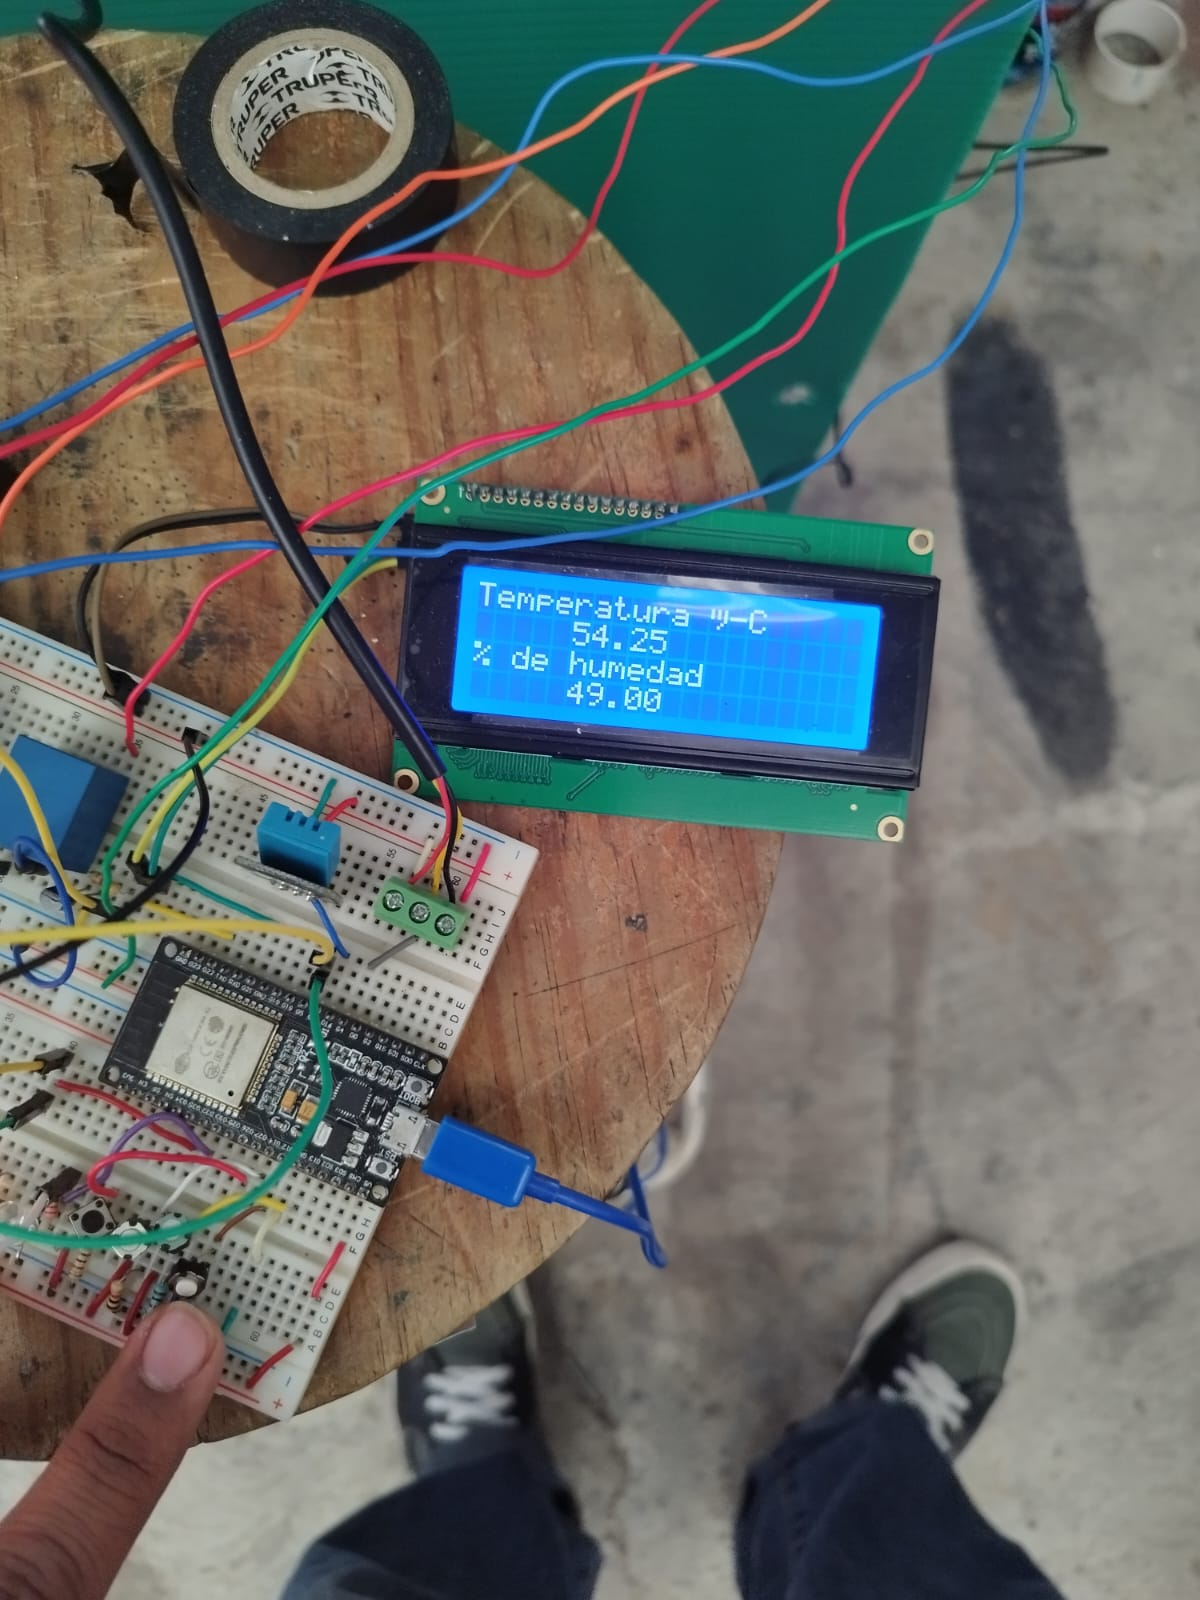
\includegraphics[scale=0.23]{images/Pruebas/Pruebas_S1/mostrar_aumento_temperatura.jpeg}
            \caption{Mostrar aumento de temperatura}
            \label{fg:botones_imp1}
\end{figure}

\clearpage

A la vez se medía el tiempo que tardaba el contenedor en calentarse, cuanto tiempo se mantenía la temperatura con el cinturón apagado y el tiempo en el que se registraba un descenso de la temperatura al interior figura (\ref{fg:botones_imp2}).

\begin{figure}[h]
            \centering
            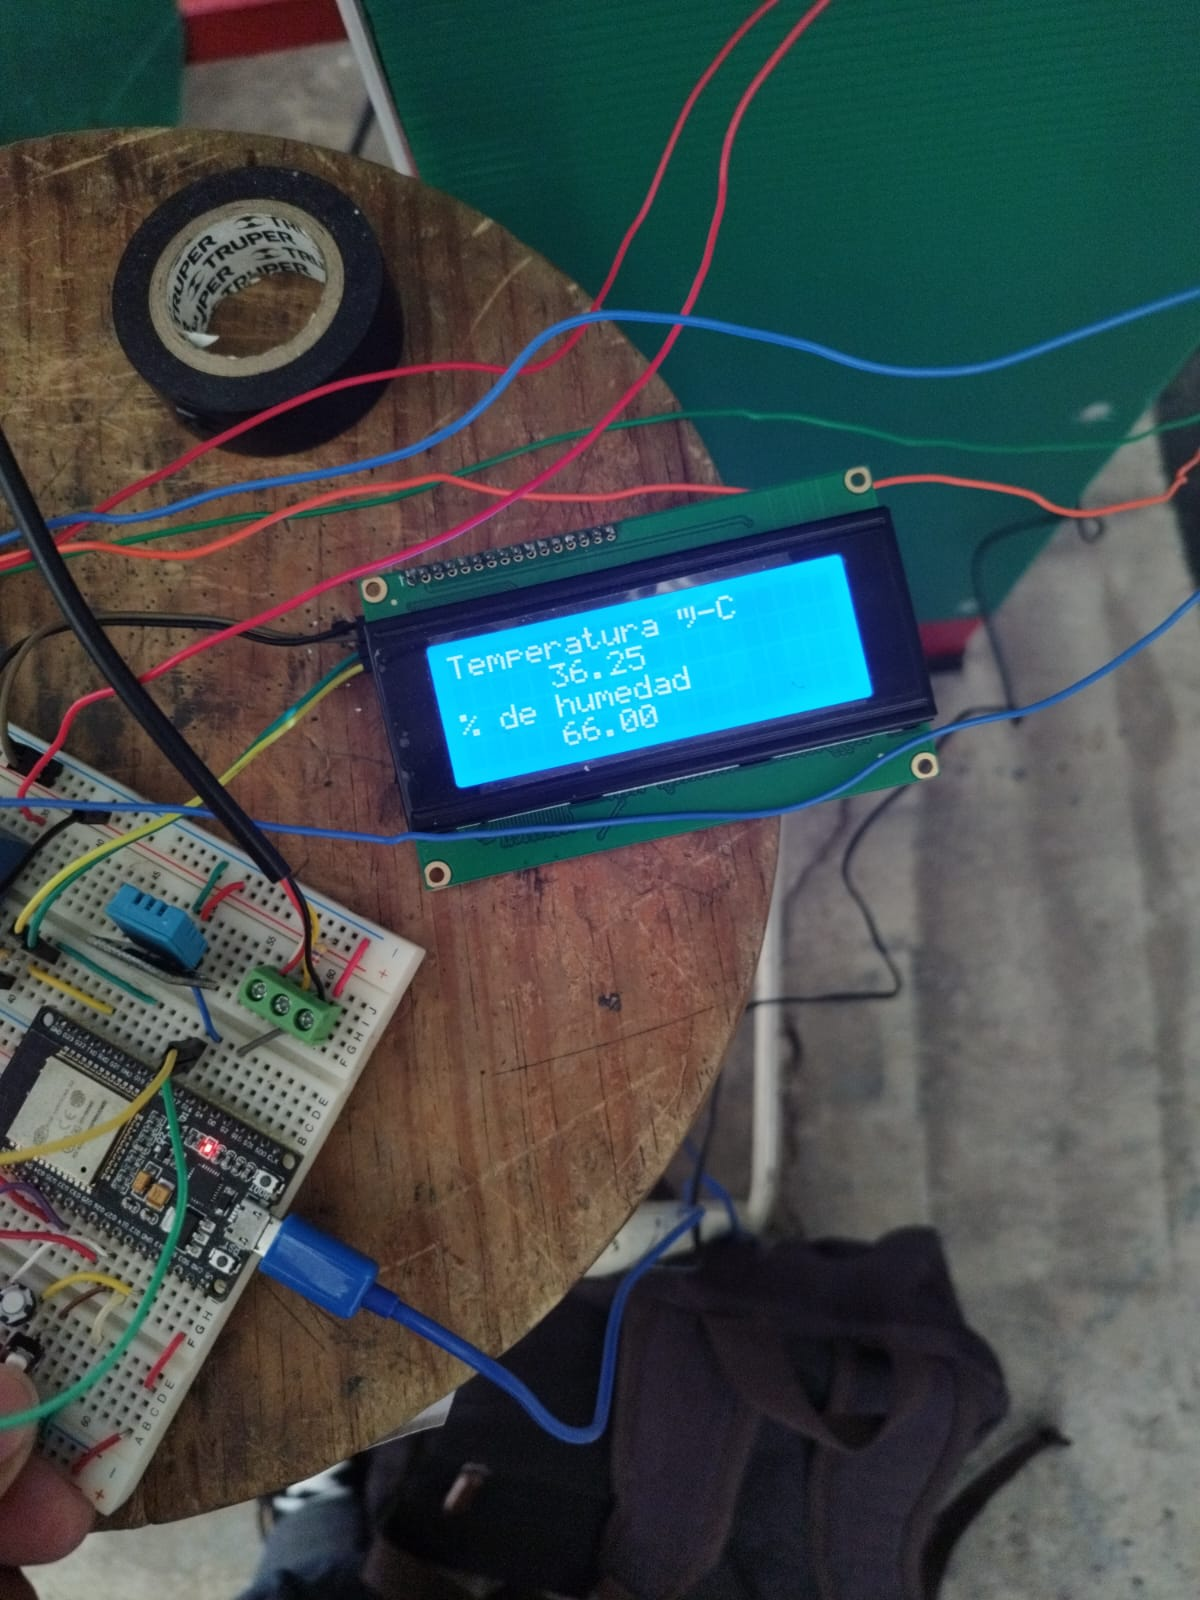
\includegraphics[scale=0.25]{images/Pruebas/Pruebas_S1/mostrar_datos.jpeg}
            \caption{Mostrar descenso de temperatura}
            \label{fg:botones_imp2}
\end{figure}

\clearpage

Para verificar el proceso, de igual manera se realizaron rutinas para corroborar que en pantalla se estuviera mostrando la etapa adecuada del compostaje figura (\ref{fg:botones_imp3}) y figura (\ref{fg:botones_imp4}).

\begin{figure}[h]
            \centering
            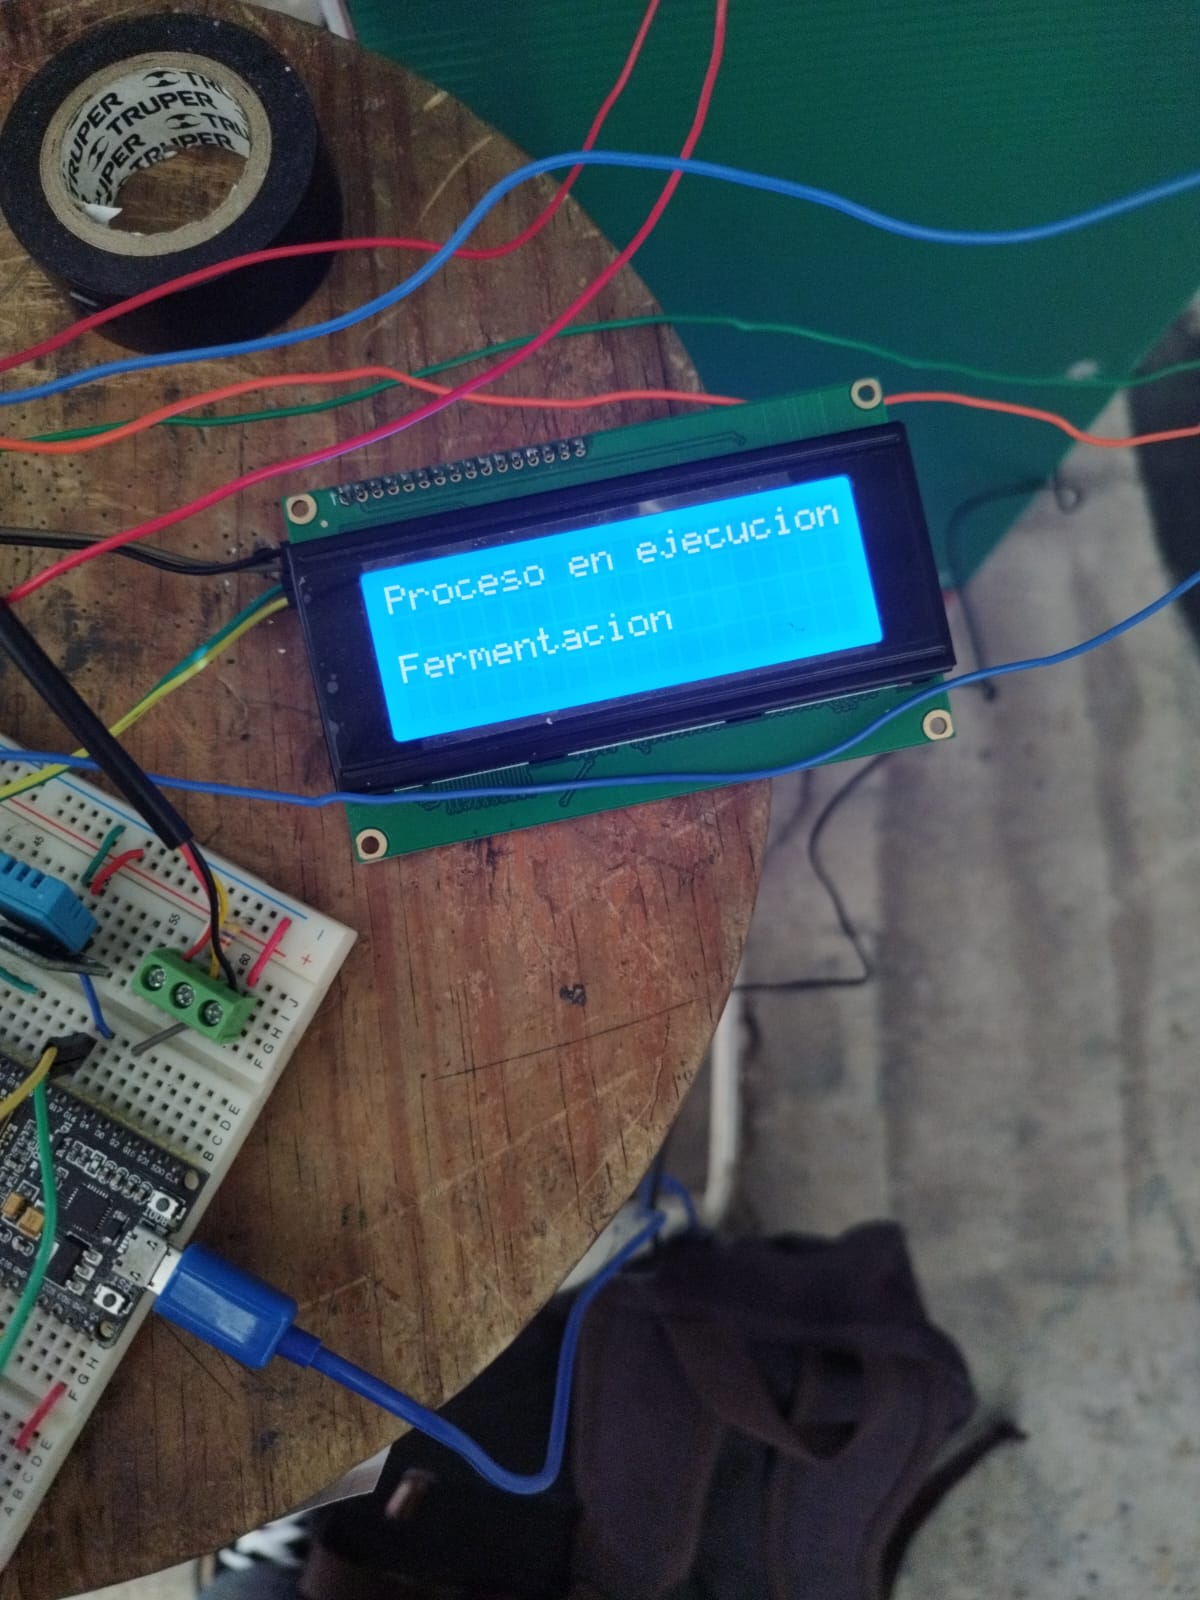
\includegraphics[scale=0.25]{images/Pruebas/Pruebas_S1/fermentacion.jpeg}
            \caption{Ejecutando fermentación}
            \label{fg:botones_imp3}
\end{figure}
\clearpage

\begin{figure}[h]
            \centering
            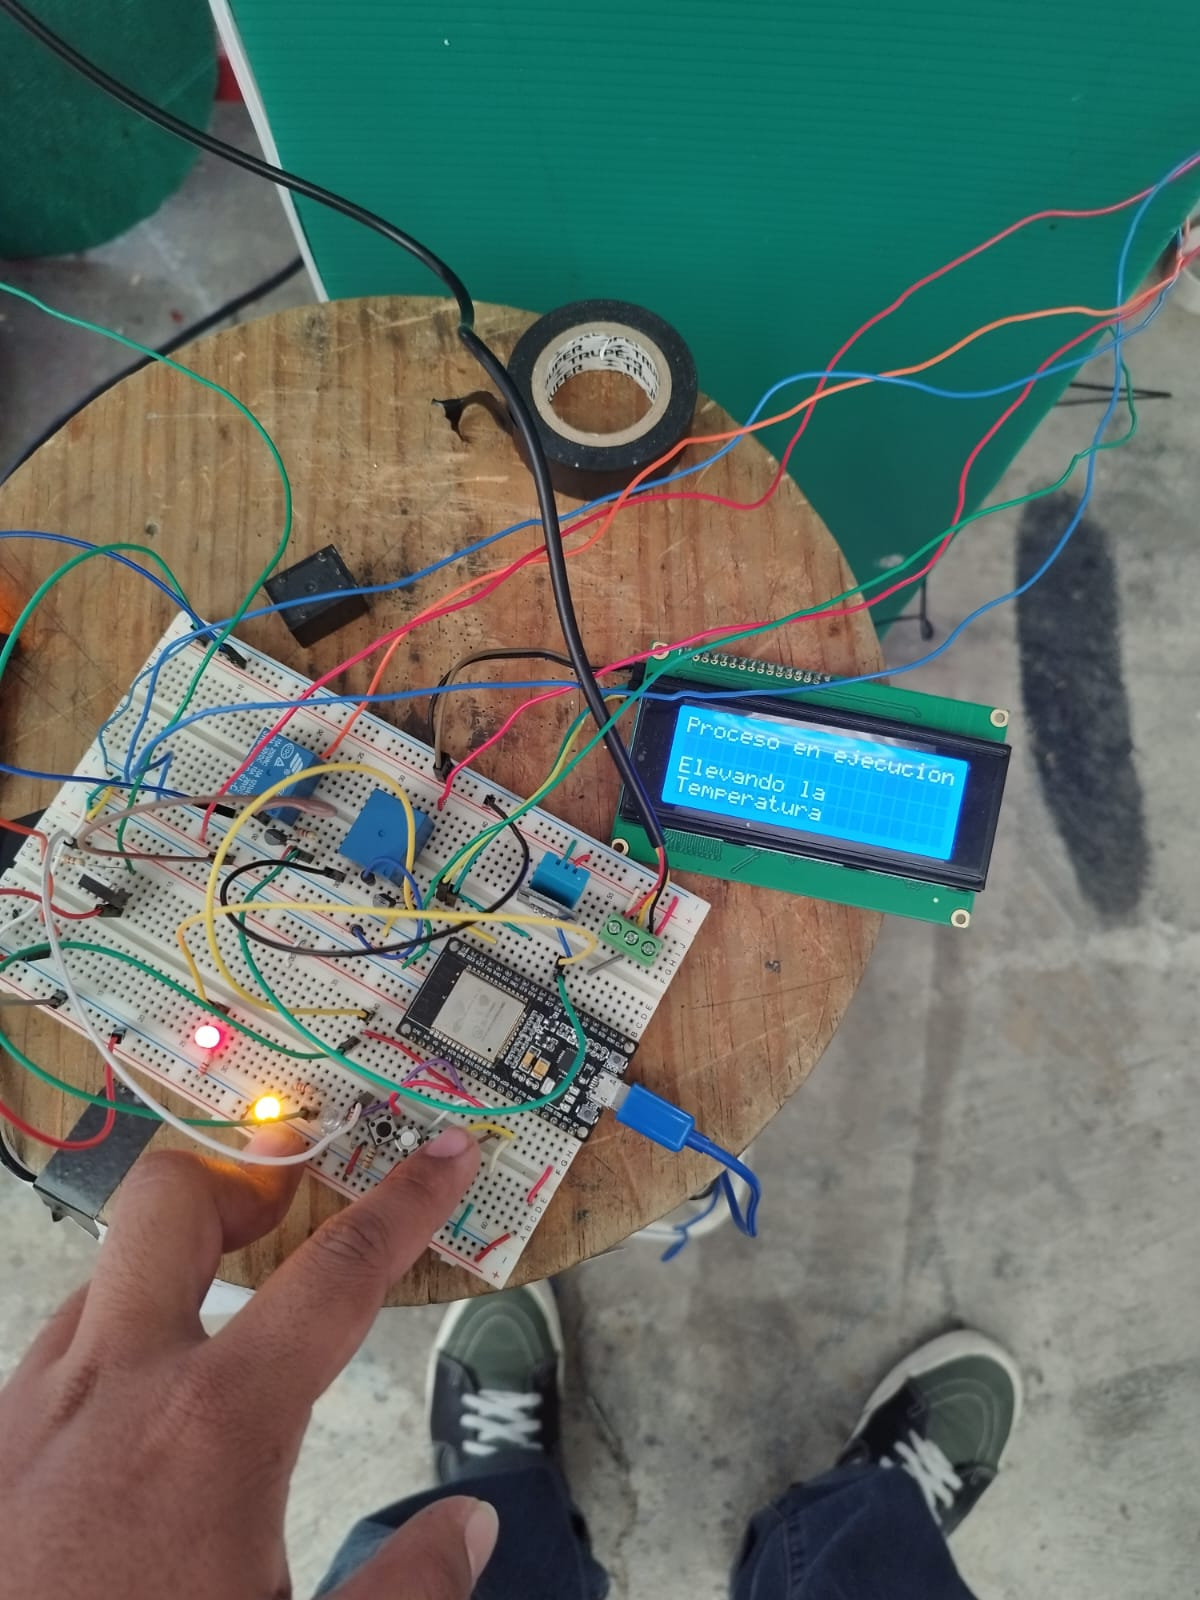
\includegraphics[scale=0.25]{images/Pruebas/Pruebas_S1/elevando_temp.jpeg}
            \caption{Ejecutando elevación de temperatura}
            \label{fg:botones_imp4}
\end{figure}

\clearpage     

Por último, para verificar que el tiempo de ejecución fuera real, se comparó la duración de ciertas rutinas con un cronómetro de celular, para comprobar que los tiempos fueran prácticamente los mismos figura (\ref{fg:botones_imp5}).

\begin{figure}[h]
            \centering
            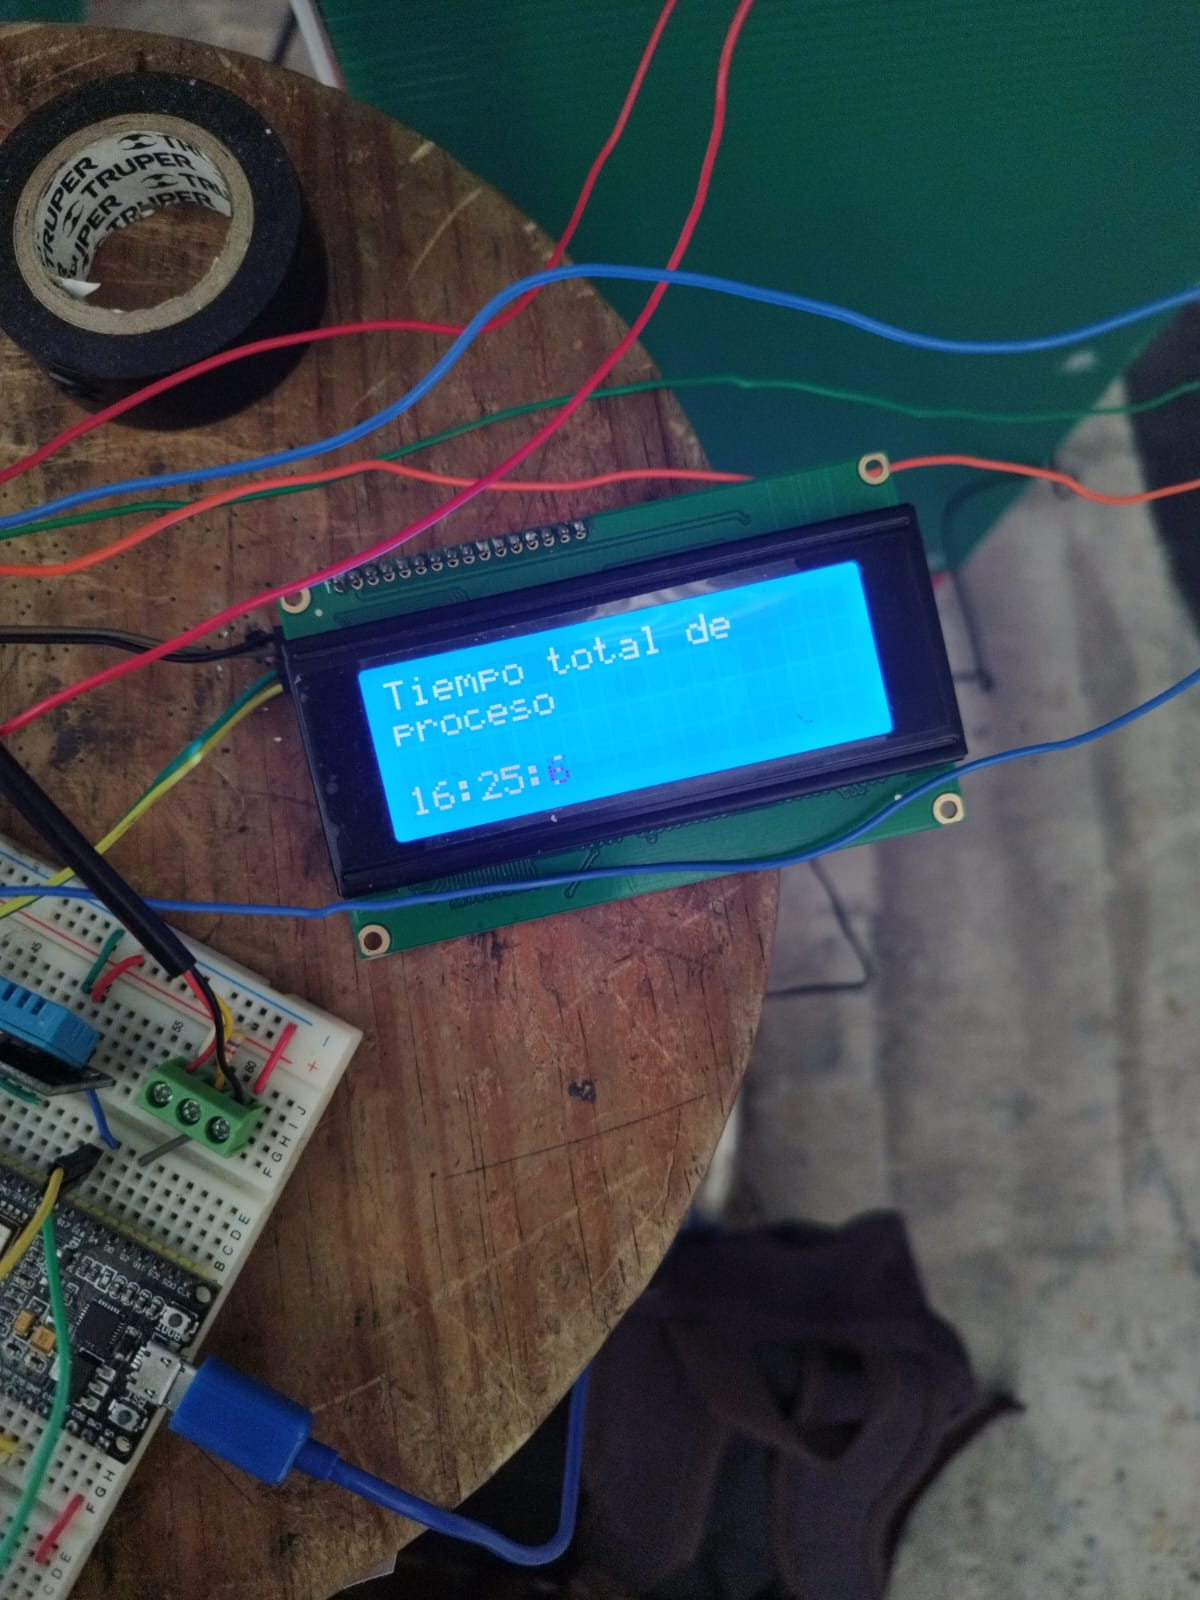
\includegraphics[scale=0.25]{images/Pruebas/Pruebas_S1/conteo_tiempo.jpeg}
            \caption{Verificación del tiempo}
            \label{fg:botones_imp5}
        \end{figure}


\clearpage



